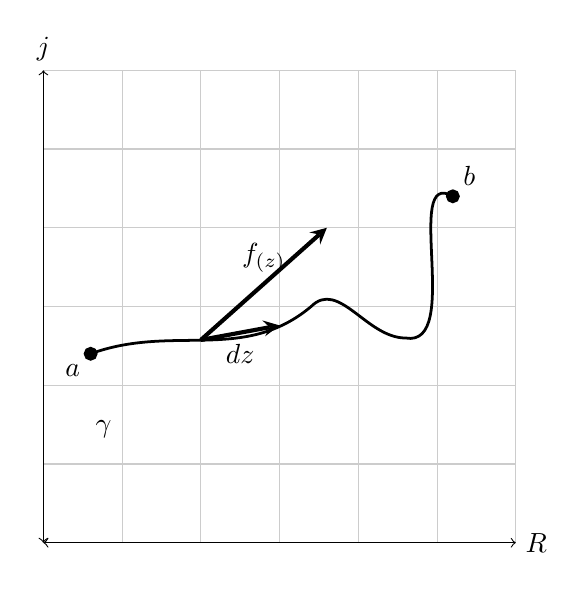
\begin{tikzpicture}[scale=2]
        \draw[step=0.5,thin,gray!40] (0,0) grid (3,3);
        \draw[<->] (0,0)--(3,0) node[right] {$R$};
        \draw[<->] (0,0)--(0,3) node[above]{$j$};
        

        \draw[line width=1pt,black] (0.3,1.2)to[out=20,in=220](1.7,1.5)to[out=45,in=180](2.3,1.3)to[out=-10,in=150](2.6,2.2);
        \draw[line width=1pt,fill=black] (0.3,1.2) circle(1pt) node[anchor=north east]{$a$};
        \draw[line width=1pt,fill=black] (2.6,2.2) circle(1pt) node[anchor=south west]{$b$};
        \draw[line width=1.5pt,-stealth] (1,1.288)--(1.8,2) node[midway, above]{$f_{(z)}$};
        \draw[line width=1.5pt,-stealth] (1,1.288)--(1.5,1.38) node[midway, below]{$dz$};
        \draw[line width=1pt] (0.5,0.6) node[anchor=south east]{$\gamma$};
         
\end{tikzpicture}
    \caption{Integral de linea sobre una curva $\gamma$}